\section{Pemodelan Sistem Tiket}
\label{apx:analisis-kebutuhan}

Untuk dapat menganalisis dan membandingkan strategi arsitektur, pertama-tama perlu didefinisikan model sistem tiket yang menjadi dasar tugas akhir. Bagian ini akan menguraikan alur kerja, komponen, serta kebutuhan fungsional dan non-fungsional dari sebuah sistem tiket acara berskala besar. Model ini dirancang untuk merepresentasikan sistem di dunia nyata dan menjadi landasan untuk mengidentifikasi titik-titik kritis yang memerlukan optimasi.

Secara umum, alur penjualan tiket untuk acara dapat dibagi menjadi tiga fase utama yang memiliki karakteristik beban yang berbeda:

\begin{enumerate}
    \item \textbf{Pemeriksaan Ketersediaan (\textit{Read-Heavy})}. Sebelum dan saat penjualan dibuka, jutaan calon pembeli secara bersamaan mengakses sistem untuk melihat informasi acara, kategori tiket, dan ketersediaan kursi. Fase ini didominasi oleh operasi baca (\textit{read}) dalam volume yang sangat masif.
    \item \textbf{Pemesanan dan Reservasi Sementara (\textit{Write-Heavy \& High Contention})}. Ini adalah fase paling kritis yang dikenal sebagai perebutan tiket. Pengguna yang berhasil menemukan tiket akan melakukan pemesanan. Sistem harus dapat menangani lonjakan operasi tulis (\textit{write}) secara bersamaan dan mengelola kondisi pacu untuk sumber daya yang sama (kursi atau kuota tiket) secara adil dan konsisten. Untuk itu, sistem umumnya menerapkan mekanisme reservasi sementara (\textit{temporary hold}) yang mengamankan tiket untuk pengguna selama jangka waktu tertentu.
    \item \textbf{Pembayaran dan Konfirmasi}. Setelah mendapatkan reservasi, pengguna melanjutkan ke tahap pembayaran. Sistem tiket harus berintegrasi secara andal dengan sistem pembayaran eksternal dan menangani konfirmasi pembayaran untuk mengubah status reservasi menjadi tiket yang sah.
\end{enumerate}

Fokus dari tugas akhir ini adalah pada fase kedua, yaitu perebutan sumber daya saat pemesanan, serta interaksinya dengan fase pertama dan ketiga. Oleh karena itu, fungsionalitas lain seperti pendaftaran pengguna (login) atau manajemen pembuatan acara oleh penyelenggara dianggap berada di luar cakupan dan tidak dimodelkan.

Berdasarkan alur tersebut, sistem yang dimodelkan terdiri dari dua komponen utama: \textbf{Layanan Tiket} sebagai sistem inti dan \textbf{Layanan Pembayaran} sebagai representasi sistem eksternal.

\subsection{Layanan Tiket}

Layanan Tiket adalah komponen sentral yang bertanggung jawab atas semua logika bisnis terkait pengelolaan acara, ketersediaan tiket, dan proses pemesanan. Layanan ini menangani semua interaksi pengguna mulai dari penjelajahan hingga konfirmasi tiket.

\subsubsection{Kebutuhan Fungsional dan Non-Fungsional}

Untuk memodelkan tantangan performa secara akurat, kebutuhan sistem didefinisikan dalam Tabel \ref{table:fungsional-tiket} untuk aspek fungsional dan Tabel \ref{table:nonfungsional-tiket} untuk aspek non-fungsional.

\pagebreak

\begingroup
\footnotesize
\begin{longtable}{|l|p{0.4\textwidth}|p{0.4\textwidth}|}
    \caption{Kebutuhan Fungsional Layanan Tiket}
    \label{table:fungsional-tiket}                                                                                                                                                                                                                                                    \\
    \hline
    \textbf{ID} & \textbf{Kebutuhan}                      & \textbf{Deskripsi}                                                                                                                                                                                                        \\
    \endfirsthead
    \multicolumn{3}{|l|}{\tablename\ \thetable\ -- \textit{Lanjutan dari halaman sebelumnya}}                                                                                                                                                                                         \\
    \hline
    \textbf{ID} & \textbf{Kebutuhan}                      & \textbf{Deskripsi}                                                                                                                                                                                                        \\
    \endhead
    \hline
    \multicolumn{3}{|r|}{\textit{Dilanjutkan ke halaman berikutnya}}                                                                                                                                                                                                                  \\
    \endfoot
    \hline
    \endlastfoot
    \hline
    \multicolumn{3}{|c|}{\textbf{Modul Penjelajahan Acara dan Ketersediaan}}                                                                                                                                                                                                          \\
    \hline
    TF-01       & Menampilkan daftar acara yang tersedia. & Sistem mampu menyajikan informasi dasar mengenai acara-acara yang sedang atau akan dijual tiketnya.                                                                                                                       \\
    \hline
    TF-02       & Menampilkan ketersediaan tiket.         & Sistem dapat menampilkan sisa kuota tiket, baik secara agregat per kategori maupun secara granular per kursi (jika berlaku), untuk sebuah acara.                                                                          \\
    \hline
    \multicolumn{3}{|c|}{\textbf{Modul Pemesanan Tiket}}                                                                                                                                                                                                                              \\
    \hline
    TF-03       & Melakukan pemesanan tiket.              & Pengguna dapat memesan satu atau lebih tiket (hingga batas tertentu, misal 5 tiket) dalam satu transaksi untuk kategori yang sama.                                                                                        \\
    \hline
    TF-04       & Mendukung jenis tiket berbeda.          & Sistem mendukung pemesanan untuk tiket dengan nomor kursi spesifik (\textit{seated}) dan tiket area berdiri bebas (\textit{free-standing}).                                                                               \\
    \hline
    TF-05       & Menerapkan reservasi sementara.         & Saat tiket dipesan, sistem akan menahannya (\textit{on-hold}) untuk pengguna selama durasi terbatas (misalnya, 15 menit) untuk memberikan waktu pembayaran. Jika pembayaran tidak selesai, tiket akan dilepaskan kembali. \\
    \hline
    \multicolumn{3}{|c|}{\textbf{Modul Manajemen Pesanan}}                                                                                                                                                                                                                            \\
    \hline
    TF-06       & Menampilkan riwayat dan status pesanan. & Pengguna dapat melihat daftar pesanan yang pernah dibuat beserta status terkininya (misal: menunggu pembayaran, berhasil, gagal).                                                                                         \\
    \hline
    TF-07       & Menangani penjualan multi-acara.        & Sistem harus mampu mengelola penjualan tiket untuk beberapa acara berbeda secara bersamaan tanpa terjadi konflik data.                                                                                                    \\
\end{longtable}
\endgroup

\pagebreak

Kebutuhan non-fungsional menjadi tolok ukur utama dalam perbandingan arsitektur karena secara langsung mendefinisikan tantangan skalabilitas dan efisiensi.

\begingroup
\footnotesize
\begin{longtable}{|l|p{0.3\textwidth}|p{0.4\textwidth}|}
    \caption{Kebutuhan Non-Fungsional Sistem Tiket}
    \label{table:nonfungsional-tiket}                                                                                                                                                                                                                   \\
    \hline
    \textbf{ID} & \textbf{Parameter}                         & \textbf{Kebutuhan}                                                                                                                                                                       \\
    \endfirsthead
    \multicolumn{3}{|l|}{\tablename\ \thetable\ -- \textit{Lanjutan dari halaman sebelumnya}}                                                                                                                                                           \\
    \hline
    \textbf{ID} & \textbf{Parameter}                         & \textbf{Kebutuhan}                                                                                                                                                                       \\
    \endhead
    \hline
    \multicolumn{3}{|r|}{\textit{Dilanjutkan ke halaman berikutnya}}                                                                                                                                                                                    \\
    \endfoot
    \hline
    \endlastfoot
    \hline
    TN-01       & Konsistensi dan Integritas Transaksi       & Sistem harus secara absolut mencegah pemesanan ganda (\textit{double booking}) untuk satu unit tiket yang sama, bahkan di bawah kondisi perebutan sumber daya yang ekstrem.              \\
    \hline
    TN-02       & Keterbaruan Data (\textit{Data Freshness}) & Data ketersediaan tiket yang ditampilkan kepada pengguna harus merefleksikan kondisi senyata mungkin untuk mengurangi pengalaman pengguna yang gagal memesan tiket yang tampak tersedia. \\
    \hline
    TN-03       & Kinerja (\textit{Performance})             & Sistem harus mampu mempertahankan latensi respons yang rendah untuk operasi baca dan laju pemrosesan pesanan (\textit{throughput}) yang tinggi selama beban puncak.                      \\
    \hline
    TN-04       & Skalabilitas dan Stabilitas                & Sistem harus dapat diskalakan untuk menangani lonjakan puluhan ribu permintaan per detik dan tetap stabil tanpa mengalami degradasi performa atau kegagalan.                             \\
\end{longtable}
\endgroup

\subsubsection{Entitas Layanan}

Untuk memenuhi kebutuhan di atas, sebuah model data relasional dirancang. Skema lengkap setiap entitas dibahas pada Lampiran \ref{apx:ticket-schema}, sedangkan gambaran umum relasi antar entitas diilustrasikan pada Gambar \ref{fig:erd-ticket-service}. Entitas utama dapat dikelompokkan menjadi dua bagian:
\begin{enumerate}
    \item \textbf{Entitas Acara dan Tiket}: Mendefinisikan struktur acara dan tiket yang dijual. Terdiri dari Event, TicketSale (periode penjualan), TicketCategory, TicketPackage, TicketArea, dan TicketSeat.
    \item \textbf{Entitas Pemesanan}: Mencatat transaksi yang dilakukan pengguna. Terdiri dari Order, OrderItem, Invoice (tagihan), dan IssuedTicket (tiket final).
\end{enumerate}

\begin{figure}[H]
    \centering
    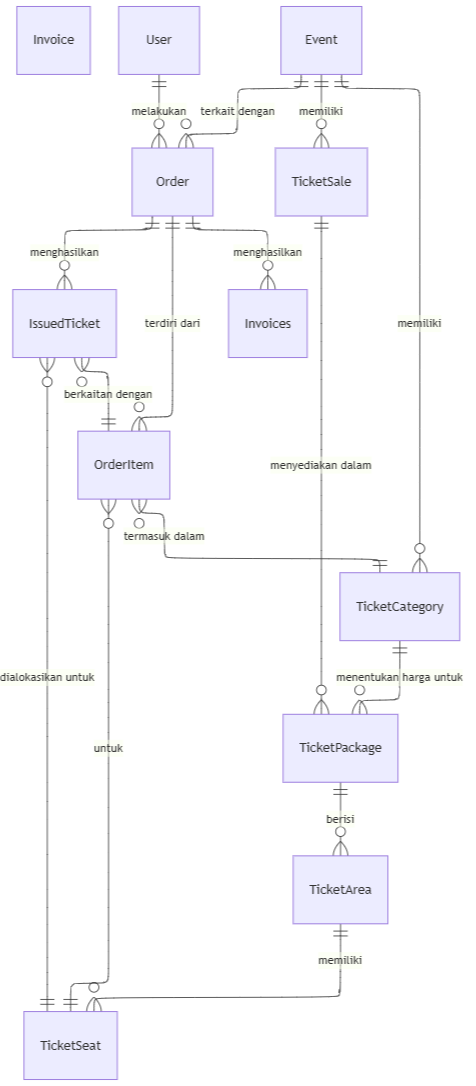
\includegraphics[width=0.65\textwidth]{resources/chapter-3/erd-mini.png}
    \caption{ERD Layanan Tiket}
    \label{fig:erd-ticket-service}
\end{figure}

Seperti yang diilustrasikan pada Gambar \ref{fig:erd-ticket-service}, entitas Order dan OrderItem menjadi pusat dari model data. Keduanya bertindak sebagai jembatan yang menghubungkan seorang User dengan Event yang spesifik, serta mengalokasikan TicketSeat yang dipesan dari TicketCategory yang tersedia.

Struktur ini memungkinkan fleksibilitas dalam penjualan. Sebuah Event bisa memiliki beberapa TicketSale (misalnya, \textit{early bird} dan penjualan umum). Setiap penjualan menawarkan beberapa TicketPackage (kombinasi kategori dan harga). Sebuah kategori bisa mencakup beberapa TicketArea (misalnya, tribun timur dan barat), dan setiap area terdiri dari banyak TicketSeat yang menjadi unit sumber daya yang diperebutkan. Status kursi (\textit{available}, \textit{on-hold}, \textit{sold}) adalah inti dari mekanisme pencegahan pemesanan ganda.

\subsection{Layanan Pembayaran}

Untuk melengkapi alur pemesanan, diperlukan integrasi dengan sistem pembayaran yang biasanya bekerja sama dengan gerbang pembayaran eksternal. Dalam tugas akhir ini, komponen ini direpresentasikan sebagai layanan eksternal tiruan (\textit{mock service}). Tujuannya adalah untuk menyimulasikan interaksi sinkron (pembuatan tagihan) dan asinkron (\textit{webhook} konfirmasi pembayaran) yang terjadi di dunia nyata, tanpa perlu menggunakan gerbang pembayaran yang sesungguhnya.

\subsubsection{Entitas Layanan}

Entitas tunggal pada layanan ini adalah Invoice (tagihan), yang merepresentasikan sebuah transaksi pembayaran. Setiap tagihan memiliki atribut esensial untuk melacak siklus hidupnya. Atribut tersebut mencakup id sebagai pengenal unik internal dan {externalId} untuk merujuk kembali ke ID pesanan pada sistem tiket. Informasi dasar seperti jumlah total tagihan (amount) dan deskripsi juga disimpan. Bagian terpenting adalah atribut status, yang dapat bernilai \textit{pending}, \textit{paid}, \textit{expired}, atau \textit{failed} untuk merefleksikan kondisi pembayaran saat ini. Terakhir, terdapat beberapa penanda waktu (\textit{timestamp}) yang krusial: createdAt mencatat kapan tagihan dibuat, expiredAt menentukan batas waktu pembayaran, dan paidAt mencatat waktu ketika pembayaran berhasil dilakukan.

\subsubsection{Kebutuhan Fungsional}

Kebutuhan fungsional layanan pembayaran yang relevan dengan sistem tiket dibahas pada Tabel \ref{table:fungsional-pembayaran}.

\begingroup
\footnotesize
\begin{longtable}{|l|p{0.4\textwidth}|p{0.4\textwidth}|}
    \caption{Kebutuhan Fungsional Sistem Pembayaran}
    \label{table:fungsional-pembayaran}                                                                                                                                                                                                   \\
    \hline
    \textbf{ID} & \textbf{Kebutuhan}               & \textbf{Deskripsi}                                                                                                                                                                   \\
    \endfirsthead
    \multicolumn{3}{|l|}{\tablename\ \thetable\ -- \textit{Lanjutan dari halaman sebelumnya}}                                                                                                                                             \\
    \hline
    \textbf{ID} & \textbf{Kebutuhan}               & \textbf{Deskripsi}                                                                                                                                                                   \\
    \endhead
    \hline
    \multicolumn{3}{|r|}{\textit{Dilanjutkan ke halaman berikutnya}}                                                                                                                                                                      \\
    \endfoot
    \hline
    \endlastfoot
    \hline
    PF-01       & Membuat tagihan pembayaran.      & Layanan dapat menerima permintaan dari sistem tiket untuk membuat sebuah tagihan baru dengan jumlah, deskripsi, dan waktu kedaluwarsa tertentu.                                      \\
    \hline
    PF-02       & Memproses notifikasi pembayaran. & Layanan dapat mengirimkan notifikasi asinkron melalui mekanisme \textit{webhook} ke sistem tiket ketika status sebuah tagihan berubah (misalnya, berhasil dibayar atau kedaluwarsa). \\
    \hline
    PF-03       & Menyediakan informasi tagihan.   & Menyediakan \textit{endpoint} bagi sistem lain untuk memeriksa status dan detail sebuah tagihan.                                                                                     \\
\end{longtable}
\endgroup
